\documentclass[conference]{IEEEtran}
\IEEEoverridecommandlockouts
\usepackage{cite}
\usepackage{amsmath,amssymb,amsfonts}
\usepackage{algorithmic}
\usepackage{graphicx}
\usepackage{textcomp}
\usepackage{xcolor}
\usepackage[english,brazilian]{babel}
\usepackage[utf8]{inputenc}
\usepackage[T1]{fontenc}
\def\BibTeX{{\rm B\kern-.05em{\sc i\kern-.025em b}\kern-.08em
    T\kern-.1667em\lower.7ex\hbox{E}\kern-.125emX}}
\begin{document}

\title{Perceptron de Múltiplas Camadas para Diagnóstico de Câncer de Mama}

\author{\IEEEauthorblockN{1\textsuperscript{o} Anara Olimpio}
    \IEEEauthorblockA{
        \textit{anaraolimpio@ig.com.br}
    }
    \and
    \IEEEauthorblockN{2\textsuperscript{o} Bruno Lopes}
    \IEEEauthorblockA{
        \textit{bruno.lopes.ti@icloud.com}
    }
    \and
}
\maketitle

\begin{abstract}
O câncer de mama é considerado o segundo tipo de câncer mais recorrente em mulheres, perdendo somente para o câncer de pele. De acordo com dados do Instituto Nacional do Câncer (INCA), em 2014, ocorreram mais de 57 mil casos de câncer de mama no Brasil em mulheres e, embora em quantidades bem pequenas, em homens. Diante do número alto de incidências, principalmente em mulheres, existe uma grande necessidade de pesquisa sobre o assunto. Este trabalho será baseado numa proposta de utilização de rede neural artificial para obter informações mais rápidas sobre o diagnóstico do câncer de mama utilizando como base para estudo e desenvolvimento do trabalho o conjunto de dados Breast Cancer Wisconsin. Este conjunto de dados de câncer de mama foi obtido do Hospital Universidade de Wisconsin, Madison, do Dr. William H. Wolberg. 

\end{abstract}

\begin{IEEEkeywords}
Perceptron. Redes Neurais Artificiais. Breast Cancer Wisconsin
\end{IEEEkeywords}
\selectlanguage{english}
\begin{abstract}
Breast cancer is considered the second most common cancer in women, losing only to skin cancer. According to data from the National Cancer Institute (INCA), in 2014, there were more than 57 thousand cases of breast cancer in Brazil in women and men (although in very small quantities). Faced with the high number of incidents, especially in women, there is a great need for research on the subject. This work will be based on a proposal to use artificial neural network to obtain faster information on the diagnosis of breast cancer using the Breast Cancer Wisconsin dataset as the basis for the study and development of the work. This breast cancer dataset was obtained from the University of Wisconsin Hospitals, Madison, by Dr. William H. Wolberg. 

\end{abstract}
\selectlanguage{brazilian}
\begin{IEEEkeywords}
Perceptron. Artificial Neural Network. Breast Cancer Wisconsin
\end{IEEEkeywords}

\section{INTRODUÇÃO}

    Esse trabalho foi construído com o intuito de praticar, experimentalmente, a utilização das redes neurais artificiais em situações reais, utilizando conjunto de dados disponíveis em portais de dados abertos, dando soluções baseadas em reconhecimento de padrões.

    Nosso trabalho iniciou-se com a escolha do conjunto de dados. Pela nossa familiaridade com o assunto referente a tumores e por entendermos que encontrar soluções que diminuam erros em diagnósticos médicos é importante, optamos por avaliar a utilização da tecnologia como facilitadora na apuração do diagnóstico do câncer de mama, através de dados extraídos de mamografias, a fim de encontrar padrões nos dados com o intuito de possibilitar a classificação dos resultados em maligno ou benigno.
    
    O conjunto de dados utilizado foi o Breast Cancer Wisconsin. Este conjunto de dados apresenta várias versões e optamos pela versão original. Sua dimensionalidade é 9, apresenta 699 registros, sendo que 16 deles apresentam erros e devem ser retirados do conjunto de dados para que isso não provoque erros no resultado.
    
    Nosso objetivo é estudar, experimentar e entender como funciona a rede neural perceptron, buscando aperfeiçoar nosso conhecimento referente a esta arquitetura e ao final do trabalho apresentamos a comparação dos resultados na utilização do perceptron com a técnica utilizada no artigo que usamos como base: An Evolutionary Artificial Neural Network Approach for Breast Cancer Diagnosis.
    
    Apresentamos, dentro desse contexto, um estudo baseado em: preparar o conjunto de dados para aplicação do perceptron, decidir pela utilização do perceptron simples ou de múltiplas camadas, normalizar os dados, separar os conjuntos de treinamento e testes, aplicar o modelo de perceptron adequado, validar os resultados.


\section{Referencial Teórico}
	%Problema, base conceitual para a solucao %
	
	Escolhemos utilizar a base de dados Breast Cancer Wisconsin, retirada do UCI Machine Learning Repository (portal com dados abertos). Esse conjunto de dados foi fornecido pelo Hospital Universidade de Wisconsin para treinar nossa Rede Neural Artificial(RNA). Esses elementos serão utilizados pela nossa Rede neural artificial, a fim aprender a classificar quais tipos de tumores são malignos e quais são benignos. 
	
	Redes neurais artificiais(RNA) são modelos inspirados na arquitetura neural do cérebro e foi desenvolvido para tentar modelar a capacidade de aprendizagem de sistemas neurais biológicos \cite{b4}. 
	
	\subsection{Perceptron Simples}
	O Modelo Perceptron foi desenvolvido nas décadas de 1950 e 1960 pelo cientista Frank Rosenblatt \cite{b9}, inspirado em trabalhos anteriores de Warren McCulloch e Walter Pitts. Hoje, é mais comum usar outros modelos de neurônios artificiais, mas o Perceptron permite uma compreensão clara de como funciona uma rede neural em termos matemáticos.
	
	
    Aprendizagem ou treinamento de rede neural artificial é equivalente a encontrar os valores de todos os pesos de tal forma que a saída desejada é gerada para a entrada correspondente, pode ser visto como a minimização da função de erro computada pela diferença entre a saída da rede e o desejado na saída de um conjunto de observações de treinamento \cite{b6}.
	
	Um Perceptron é um modelo matemático que recebe várias entradas, x1, x2, … xn e produz uma única saída binária, forme monstra na Figura 1.
	
	\begin{figure}[htbp]
	\centerline{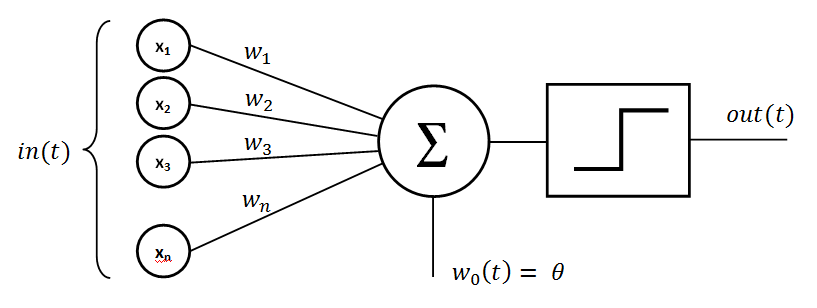
\includegraphics[scale=1]{Perceptron.png}}
	\caption{Perceptron simples}
	\label{fig}
	\end{figure}
	
	No exemplo ilustrado na Figura 2, o Perceptron possui n entradas: x1, x2, … xn. Rosenblatt propôs uma regra simples para calcular a saída. Ele introduziu pesos, w1, w2, …, números reais expressando a importância das respectivas entradas para a saída. A saída do neurônio, 0 ou 1, é determinada pela soma ponderada, menor ou maior do que algum valor limiar (threshold) \cite{b9}. Assim como os pesos, o threshold é um número real que é um parâmetro do neurônio. Em termos algébricos temos:
	
	\begin{figure}[htbp]
	\centerline{
\includegraphics[scale=0.8]{Perceptron-threshold.png}}
	\caption{Soma Ponderada com threshold}
	\label{fig}
	\end{figure}

    O Perceptron é um classificador linear (binário). Além disso, é usado na aprendizagem supervisionada e pode ser usado para classificar os dados de entrada fornecidos.
    
    Um único Perceptron consegue resolver somente funções linearmente separáveis,  mas como nosso modelo de dados tem características não linear, como podemos ver na Figura 3, o Perceptron não consegue gerar um hiperplano para separar os dados. Por isso buscamos uma variante do modelo de Perceptron simples, o Perceptron de Múltiplas Camadas.
    
    \begin{figure}[htbp]
	\centerline{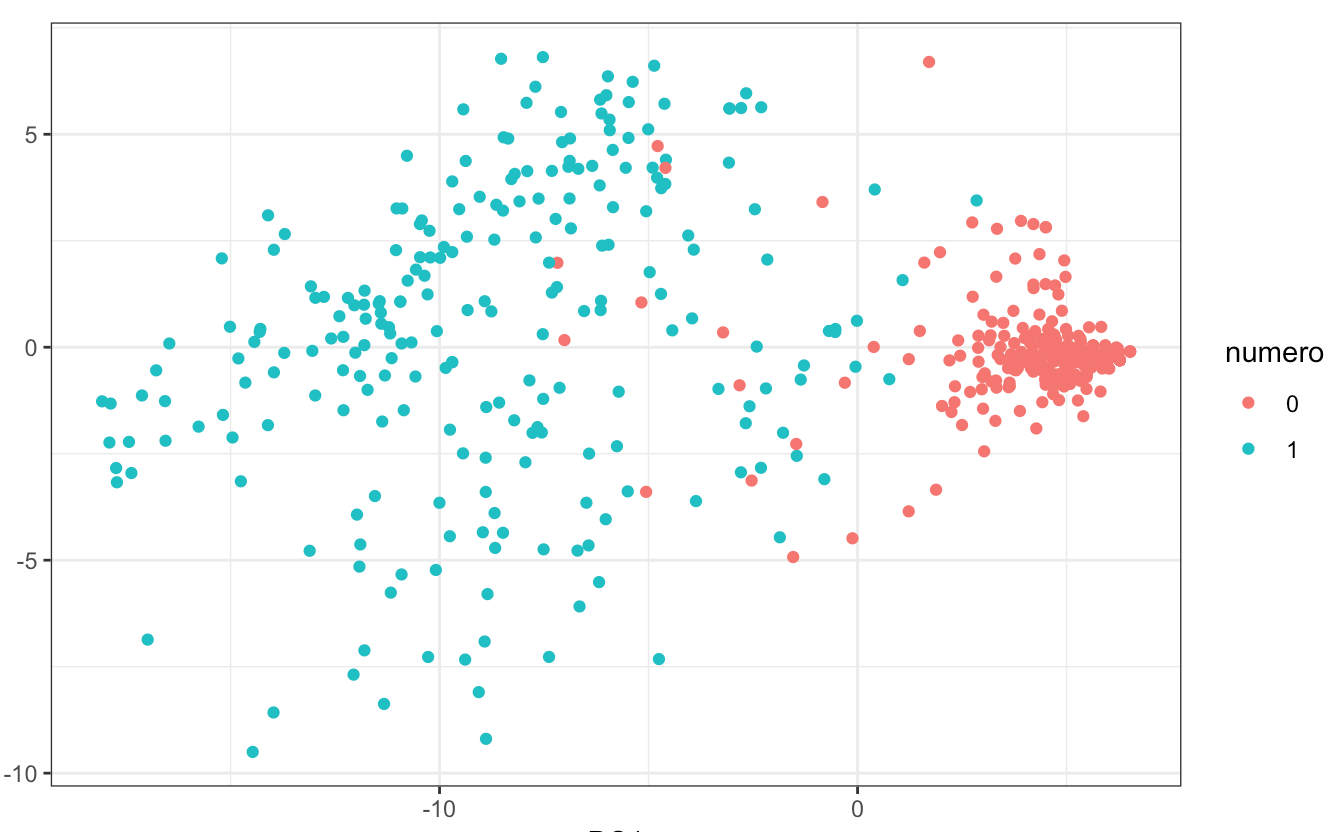
\includegraphics[scale=0.3]{dados-cancer.png}}
	\caption{Amostra dos dados (0 = benigno, 1 = maligno)}
	\label{fig}
	\end{figure}
    
    \subsection{Perceptron de Múltiplas Camadas (MLP)}
    Um Perceptron de Múltiplas Camadas é uma variante do modelo Perceptron original proposto por Rosenblatt na década de 1950 \cite{b9}. Tem uma ou mais camadas escondidas entre suas camadas de entrada e saída. Uma arquitetura típica de rede neural artificial conhecida como Perceptron de Múltiplas Camadas (MLP) contém uma série de camadas, compostas de neurônios e suas conexões \cite{b14}. Um neurônio artificial tem a capacidade de calcular a soma ponderada de suas entradas e, em seguida, aplica uma função de ativação para obter um sinal que será transmitido para o próximo neurônio. Os neurônios são organizados em camadas, as conexões são sempre direcionadas de camadas inferiores para camadas superiores, os neurônios na mesma camada não estão interligados, conforme ilustrado na Figura 4.
    
    \begin{figure}[htbp]
	\centerline{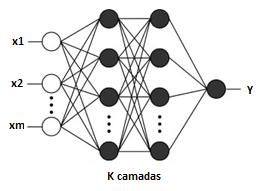
\includegraphics[scale=1.2]{Perceptron-Multicamadas.png}}
	\caption{Perceptron Multicamadas}
	\label{fig}
	\end{figure}
    
    A definição da arquitetura em redes MLP é um ponto muito relevante, a falta de conexões pode tornar a rede incapaz de resolver o problema de parâmetros ajustáveis, enquanto um excesso de conexões pode causar um ajuste excessivo dos dados de treinamento \cite{b7}.

    \subsection{Base de Dados}

    O banco de dados utilizado nesse experimento foi obtido da Universidade de Wisconsin Hospitals \cite{b10} \cite{b11}. Os atributos 2 a 10 foram usados para representar instâncias. Cada instância tem uma das duas classes possíveis: benigna ou maligna.
    
    As amostras foram coletadas periodicamente, enquanto o Dr. Wolberg relatava seus casos clínicos \cite{b12}. 
    O banco de dados, portanto, reflete esse agrupamento cronológico dos dados.
    Esta informação de agrupamento aparece imediatamente abaixo, tendo sido removida    dos dados em si:

\begin{description}
     \item Grupo 1: 367 instâncias (janeiro de 1989)
     \item Grupo 2: 70 instâncias (outubro de 1989)
     \item Grupo 3: 31 instâncias (fevereiro de 1990)
     \item Grupo 4: 17 instâncias (abril de 1990)
     \item Grupo 5: 48 instâncias (agosto de 1990)
     \item Grupo 6: 49 instâncias (janeiro de 1991)
     \item Grupo 7: 31 instâncias (junho de 1991)
     \item Grupo 8: 86 instâncias (novembro de 1991)
\end{description}
    No total, são 699 (a partir da base de dados doada em 15 de julho de 1992) \cite{b10} \cite{b11}. Observe que os resultados resumidos acima, em uso, referem-se a um conjunto de dados, inicialmente,   de tamanho 369, enquanto o Grupo 1 tem apenas 367 instâncias. Isso porque, originalmente, continha 369 instâncias e 2 foram removidas. 
   
   Temos no total 10 atributos mais a classe, conforme apresentado na Tabela I.
    
    \begin{table}[h]
	\caption{Descrição base de dados Wisconsin}
	\begin{center}
    \begin{tabular}{l | c }
    \hline
       Descrição do atributos & Valores \\\hline
       Clump Thickness & 1 a 10 \\\hline
       Uniformity of Cell Size & 1 a 10 \\\hline
       Uniformity of Cell Shape & 1 a 10 \\\hline
       Marginal Adhesion & 1 a 10 \\\hline
       Single Epithelial Cell Size & 1 a 10 \\\hline
       Bare Nuclei & 1 a 10 \\\hline
       Bland Chromatin & 1 a 10 \\\hline
       Normal  & 1 a 10 \\\hline
       Mitoses & 1 a 10 \\\hline
       Classe &(2 for benign, 4 for malignant)\\\hline
    \end{tabular}
    \end{center}
    \end{table}
    

    Existem 16 registros com dados inválidos dentro do arquivo, eles vieram com o caracter '?'  no campo Bare Nuclei e consequentemente tivemos eliminalos. Com isso, ficamos com a seguinte distribuição para treinamento e testes: Benigno: 458 (65.5\%) Maligno: 241 (34.5\%)

	
	
\section{Preparação dos dados para o treinamento}
    % Metodologia, experimentos e resultados, analise dos resultados(porques) %
    
    Em primeiro momento, fizemos um trabalho de ajustes simples do conjunto de dados para que os mesmos estivessem prontos para a aplicação do modelo. 
    
    Precisamos excluir a coluna do código de identificação do registro pois não traziam informações relevantes para nosso trabalho e transformamos o atributo Classe em uma coluna de saída(Y) em dados binários (0 para benigno e 1 para maligno). 
    
    Antes de realizar o treinamento sobre o conjunto de dados, precisamos remover alguns registros que vieram com dados incorretos, um total de 16 registros que estavam com sinal '?' na coluna 7 - Bare Nuclei, fizemos isso, para que o resultado final não fosse prejudicado, pois alguns valores vieram sem dados. Ao final ficamos com a seguinte distribuição: Maligno 241 e Benigno 458.
    
    Num segundo momento, precisamos entender qual tipo de Perceptron nos atenderia. 
    
    Inicialmente, pensamos em utilizar perceptron simples para tentar classificar nossa base de dados, mas entendemos que dificilmente conseguimos encontrar no mundo real elementos cuja caraterística é não linear. Para constatarmos qual tipo de perceptron deveríamos utilizar (simples ou de múltiplas camadas), foi criado um gráfico que demonstrasse se o nosso conjunto de dados era linearmente separável ou não. Para isso, utilizamos a técnica da análise de componentes principais (PCA), conforme figura 3, com isso, constatamos que o conjunto de dados utilizado em nossos experimentos é de caráter não linear e então tivemos que buscar outra heurística.
    
    Na busca por uma solução que atendesse as nossas necessidades, entendemos que precisaríamos utilizar a arquitetura de rede neural Perceptron de Múltiplas Camadas. Esse modelo tem uma ou mais camadas escondidas de neurônios e é diferente do perceptron simples, consegue treinar, testar e aprender sobre dados não lineares.
    
    \subsection{Topologia da rede Perceptron Multicamadas}
    
    A definição da arquitetura em redes Perceptron de Múltiplas Camadas é um ponto muito relevante, porque por um lado, se utilizamos muitas conexões podemos ter um ajuste excessivo dos dados de treinamento, por outro lado, a falta de conexões pode fazer com que a rede não seja capaz de resolver o problema de parâmetros ajustáveis \cite{b7}.

    O design das camadas de entrada e saída da nossa rede é direto. Por exemplo, como estamos tentando ensinar nossa rede a classificar tumores malignos e benignos, uma maneira natural de projetar a rede é codificar o número de classes (9 classes existentes na base de dados) nos neurônios de entrada. A camada de saída conterá apenas um único neurônio com valores inferiores a 0,5 indicando que  o tumor é benigno e valores maiores que 0,5 indicando que o tumor é maligno.
    
\subsection{Preparação par treinamento do modelo}
     Utilizamos a função MLP já disponível no R. Essa função cria, treina e testa, automaticamente, um perceptron de múltiplas camadas. 
     
     Antes da aplicação do treinamento, precisamos ainda, normalizar os dados de entrada, todos nossos registros estavam classificados com valores de 0 a 10, a normalização facilita o treinamento do modelo. a normalização transforma os dados entre 0 e 1.
     
     Quando treinamos nosso modelo em um conjunto de dados (conjunto de dados de treinamento) e testamos o desempenho de nosso modelo em outro conjunto de dados (conjunto de dados de teste), a medida de desempenho usando o conjunto de dados de teste é conhecida como acurácia, podemos encontrar dados para o cálculo da acurácia através da matrix de confusão que fazemos em cima do resultado da função MLP, citada acima.
    
    Para conseguir medir a acurácia da nossa rede precisamos dividir o conjunto de dados em treinamento e teste. O conjunto de treinamento contém os dados da mesma classe dos dados de treinamento, com exemplos rotulados em malignos e benignos. Este conjunto é para construir nosso modelo. O modelo aprende com os elementos de treinamento e é avaliado com os elementos do teste. Com isso podemos verificar se a nossa rede consegue generalizar e aprender.
    
    Para esse experimento dividimos nosso conjunto de dados de acordo com a seguinte regra: 80/20, ou seja, 80\% do conjunto de dados vai para o conjunto de treinamento e 20\% para o conjunto de testes. 
    
    Para que obter um conjunto de teste homogêneo, realizamos a seguinte operação:
    
    \begin{itemize}
    
    \item Passo 1: Carregamos todos todo conjunto de dados;
    \item Passo 2: Pegamos os 10 primeiros registros
    \item Passo 3: 2 primeiros itens para teste
    \item Passo 4: Itens restantes para treinamento
    \item Passo 5: Repetir passo 2 até que todos os registros sejam distribuídos
    
    \end{itemize}
    
   Resultou no seguinte cenário de distribuição: 544 registros para treinamento e 138 para teste. A separação de 10 em 10, de forma intercalada, é importante para temos uma distribuição mais uniforme das coletadas em momentos diferentes no treinamento e teste, já que os dados foram coletados em ordem cronológica como visto anteriormente.
    
    
  
   \subsection{Treinamento e resultados}
    
    Ao final do treinamento a topologia apresentada, conforme Figura 5 apresentou os melhores resultados tanto no conjunto de dados de treinamento e como no conjunto de teste. 
    
    Particularmente, não é possível resumir o processo de design das camadas ocultas com poucas regras. 
    
        \begin{figure}[htbp]
	\centerline{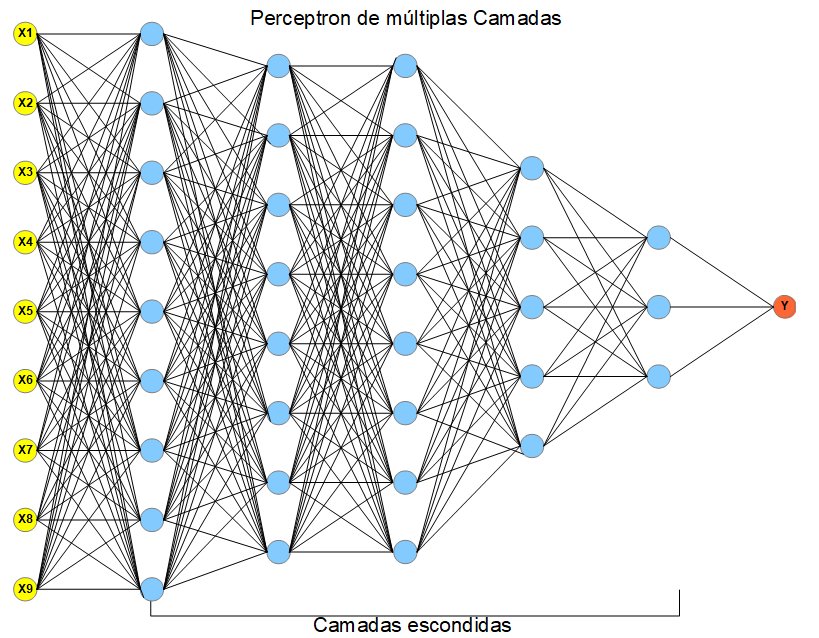
\includegraphics[scale=0.4]{Perceptron-MLP.png}}
	\caption{Topologia Perceptron de Múltiplas Camadas}
	
	\label{fig}
	\end{figure}
    
   Dados utilizados no treinamento e testes:
    
     \begin{itemize}
    
    \item Função: MLP;
    \item Taxa de aprendizado: 1;
    \item Número de iterações: 10.000;
    \item Camadas escondidas: 5;
    \item Valores de neurônios em cada camada escondida: 9, 8, 8, 5 e 3;
    \item  Inicialização dos pesos: Aleatória;
    
    \end{itemize}
  
  Depois de determinar o número ideal de camadas ocultas, taxa de aprendizado e números de iterações tivemos os seguintes resultados nos momentos de treinamento e testes(tabela II):
     
    \begin{table}[h]
	\caption{Resultado dos testes}
	\begin{center}
    \begin{tabular}{l | c | r }
    \hline
         \# Iterações &Acurácia trenamento  & Acurácia teste \\\hline
         50 &97.42647  &95.65217    \\\hline
         100 &98.88268  &95.65217    \\\hline
         1000 &99.44341  &96.37681    \\\hline
         10000 &99.08088  &97.10145   \\\hline
         20000 &99.26471  &97.10145  \\\hline
    \end{tabular}
    \end{center}
    \end{table}
     
    
    Podemos observar que os resultados de classificação obtidos dos dados de teste mostrados foram bons, porque tivemos uma acurácia alta, mesmo para testes onde o número de ciclos foi pequeno como apresentado na Tabela II.
    
    As Figuras 6 e 7 ilustram a retropropagação do erro de dois experimentos.
    
    \begin{figure}[htbp]
	\centerline{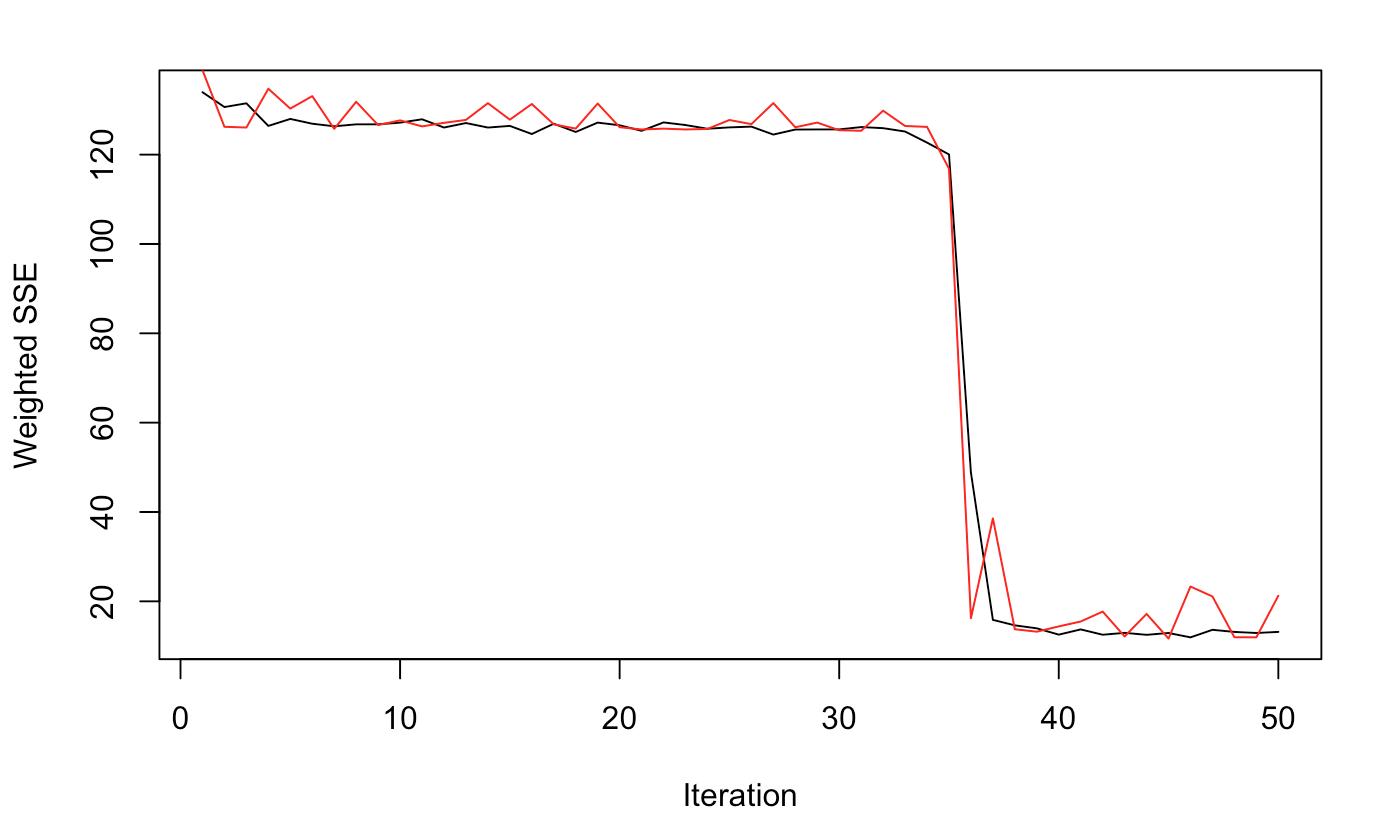
\includegraphics[scale=0.4]{imagens/9,8,8,5,3-50.png}}
	\caption{Função de Custo 50 iterações}
	
	\centerline{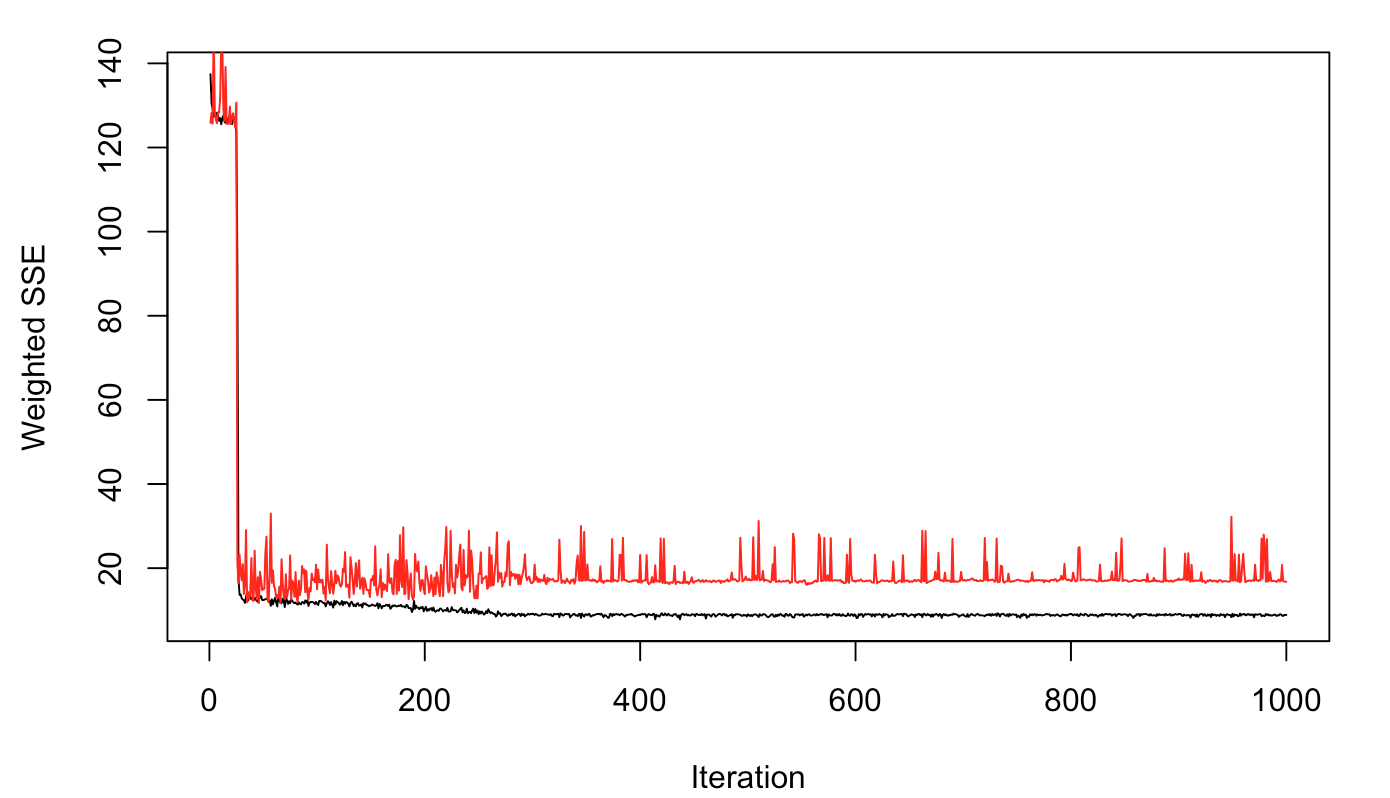
\includegraphics[scale=0.4]{imagens/9,8,8,5,3-1000.png}}
	\caption{Função de Custo 1000 iterações}
	\label{fig}
	\end{figure}
	
	 O retropropagação é a técnica de rede neural mais utilizada no reconhecimento de padrões, consiste na utilização dos pesos, considerando a propagação do erro de saída da rede para a sua entrada. Este algoritmo também é conhecido como regra delta generalizada \cite{b12} \cite{b13}. 
	 
	 A demonstração de resultados através de gráficos é relevante, pois nos dá uma visão mais clara no alcance dos objetivos do treinamento e teste. 
	 
	 As Figuras 8 e 9 nos mostram o resultado do treinamento em forma de gráfico:
	 
	 
    \begin{figure}[htbp]
	\centerline{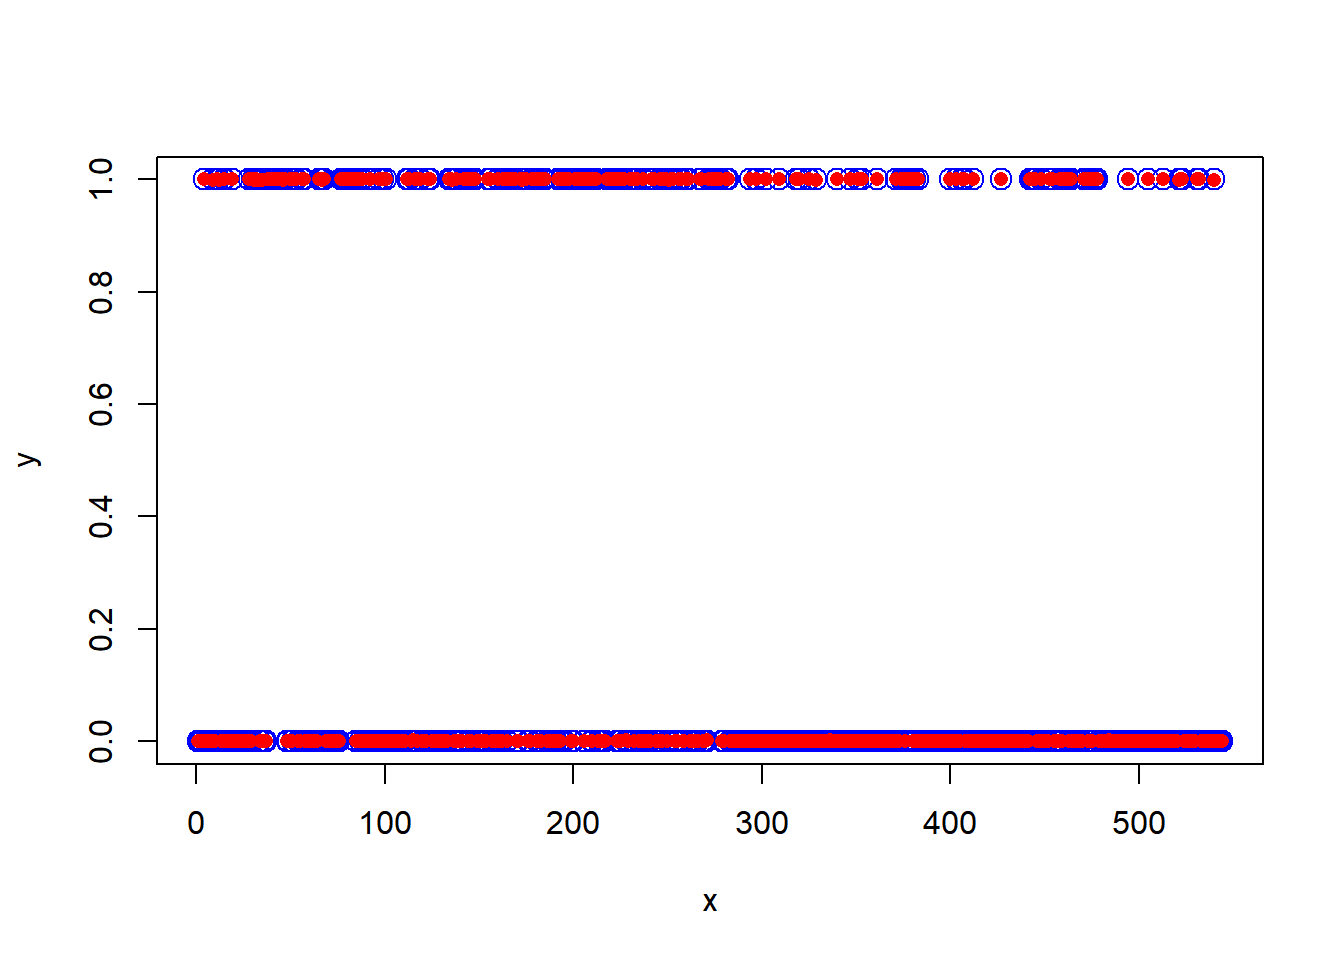
\includegraphics[scale=0.15]{grafico-treinamento.png}}
	\caption{Resultado do treinamento}
	
	\label{fig}
	\end{figure}
	
    \begin{figure}[htbp]
	\centerline{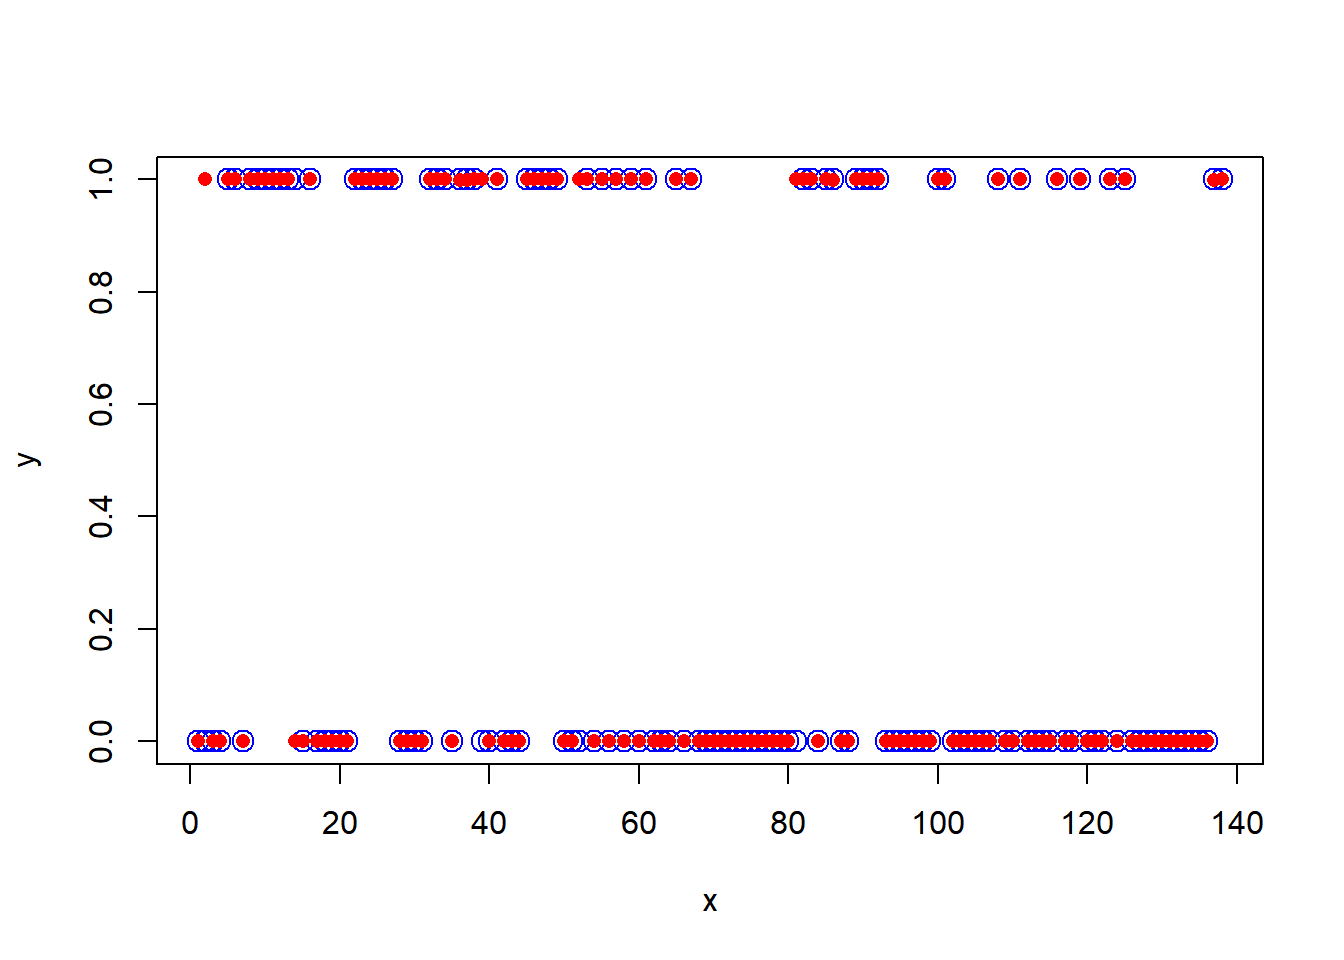
\includegraphics[scale=0.15]{grafico-teste.png}}
	\caption{Resultado do teste}
	
	\label{fig}
	\end{figure}
	
\section{Resultado e Discussão}

    No nosso estudo, utilizamos o Perceptron de Múltiplas Camadas(MLP), conseguimos uma precisão de 97,10\% e para isso precisamos de 10.000 épocas, conforme apresentado na Tabela II.
    
    Ao analisar a retropropagação do erro Figura 6 e 7 e comparar com os resultados apresentados na Tabela II, verificamos que com apenas 50 épocas conseguimos uma acurácia de 95,65\%, após isso, temos pouca variância estatística.
    
    O limite máximo de acurácia atingido em nossos estudos foi 97,10\%. Mesmo alterando o número máximo de iterações, não conseguimos melhorar a precisão conforme apresentado na Tabela II.

    No artigo An Evolutionary Artificial Neural Network Approach for Breast Cancer Diagnosis, utilizado como base para nossos estudos, foi apresentado uma proposta de utilização do algoritmo genético adaptativo (AGA), aplicado para evoluir a rede neural de propagação reversa (BP). Esse experimento conseguiu alcançar uma precisão de classificação de 98,9\% com 1000 épocas \cite{b1}. Verificamos que esse resultado, utilizando computação natural, é muito significante e traz uma precisão muito alta. 

    Após finalizar nossos experimentos, verificamos que nossos resultados foram inferiores ao apresentado pelo algoritmo genético adaptativo \cite{b1}.
    
    Não fizemos incremento aos dados do artigo utilizado como base, pois nosso objetivo era compreender o funcionamento do perceptron e ao fim poder comparar os resultados alcançados com o artigo utilizado como referência.
    
    
\section*{Conclusão}

  No decorrer do trabalho podemos perceber que o assunto está sendo bastante abordado por muitos outros pesquisadores e isso nos dá uma satisfação muito grande, por perceber que tem muitos estudos feitos na área da medicina utilizando a aprendizagem de máquina, entendemos que esse assunto traz uma contribuição muito grande não só na eficiência para encontrar diagnósticos mais precisos mas também para prever ocorrências importantes como uma situação epidemiológica, por exemplo.
  
  Com relação ao nosso trabalho, especificamente, podemos concluir que os experimentos foram satisfatórios, porém tivemos bastante trabalho para chegar ao resultado final, acreditamos que isso tenha ocorrido por falta de conhecimento previo nessa área e que a experiência nos ajudaria muito nas etapas do processo e essas foram as maiores dificuldades enfrentadas também.
  
  Pelos motivos citados, passamos muito tempo trabalhando sobre o modelo, porém, entendemos que nosso aprendizado foi bem interessante. Para chegarmos no resultado final tivemos que conhecer e entender todos os passos do treinamento e teste de um aprendizado de máquina, o que é muito importante para o nosso objetivo dentro do curso.
 
    
    O assunto que precisamos aprender sozinhos foi como demonstrar graficamente se os dados que estamos utilizando são linearmente separáveis ou não para entendermos qual tipo de perceptron atenderia nosso experimento. Nosso conjunto de dados tem dimensionalidade 9 e nos deparamos com a dificuldade da plotagem utilizando os mesmos recursos que vínhamos desenvolvendo nos nossos trabalhos semanais, para isso, precisamos aprender a utilizar o PCA(Principal Component Analysis). Ao buscar informações sobre o assunto, deparamos com a quantidade infinita de materiais na área de inteligência artificial que podem nos auxiliar no desenvolvimento e entendimento de assuntos diversos nesse ramo.
    
    Referente à nossa opinião de potencialidade para publicar o trabalho, acreditamos que para que um trabalho seja publicável ele tem que trazer informações novas e resultados bastante relevantes, tais como: um conjunto de dados que foi criado pelos autores ou uma melhoria num algoritmo existente, criação de um algoritmo que melhore, sistematicamente, a aprendizagem cognitiva ou que seja novo no mercado e baseado nessas considerações, entendemos que o nosso trabalho não apresenta requisitos para publicação, pois foi baseado em soluções anteriores existentes.
    


\begin{thebibliography}{00}

\bibitem{b1} AN EVOLUTIONARY ARTIFICIAL NEURAL NETWORK APPROACH FOR BREAST CANCER DIAGNOSIS. Washington: Third International Conference on Knowledge Discovery and Data Mining, 2010. Anual. ISBN: 9781424463979.

\bibitem{b13} Bishop, C.M.: “Neural Networks for Pattern Recognition”. Oxford University Press,New York (1999).

\bibitem{b12} Duda, R.O., Hart, P.E.: “Pattern Classification and Scene Analysis”, In: Wiley-Interscience Publication, New York (1973)

\bibitem{b2} Livraria digital do Instituto de Engenheiros Eletricistas e Eletrônicos (IEEE), AN EVOLUTIONARY ARTIFICIAL NEURAL NETWORK APPROACH FOR BREAST CANCER DIAGNOSIS, disponível em https://ieeexplore.ieee.org/document/5432472, acesso em 20 de setembro de 2018.

\bibitem {b6} M. Ettaouil and Y. Ghanou, “Neural architectures optimization and Genetic algorithms”, Wseas Transactions On Computer, Issue 3, Volume 8, 2009, pp. 526-537. 

\bibitem{b10} O. L. Mangasarian and W. H. Wolberg: "Cancer          diagnosis via linear 
      programming", SIAM News, Volume 23, Number 5, September 1990, pp 1 & 18.

\bibitem{b3} Pfizer, industria farmacêutica, O câncer de mama em números no Brasil e no mundo, disponível em https://www.pfizer.com.br/noticias/Cancer-de-mama-em-numeros, acesso em 15 de setembro de 2018.

\bibitem{b5} Ramchoun H, Amine M, Idrissi J, Ghanou Y, Ettaouil M. Multilayer Perceptron: Architecture Optimization and Training. International Journal of Interactive Multimedia and Artificial Intelligence. 2016;4(1):26–30.

\bibitem{b9} Rosenblatt, “The Perceptron: A Theory of Statistical Separability in Cognitive Systems”, Cornell Aeronautical Laboratory, Report No. VG1196-G-1, January, 1958. 

\bibitem{b4} Salchenberger LM, Cinar E, Lash NA. Neural networks: A new tool for predicting thrift failures. Decision Sciences. 1992;23(4):899–916

\bibitem{b14} S. Haykin, Redes Neurais: Princípios e prática, Bookman, 2. ed., 2001.

\bibitem {b7} T.B Ludermir “Hybrid Optimization Algorithm for the Definition of MLP Neural Network Architectures and Weights” Proceedings of the Fifth International Conference on Hybrid Intelligent Systems (HIS’05) 0-7695- 2457-5/05 20.00 2005 IEEE.

\bibitem{b8} UCI Machine Learning Repository, Breast Cancer Wisconsin, disponível em http://archive.ics.uci.edu/ml/datasets/Breast+Cancer+Wisconsin+(Original), acesso em 25 de agosto de 2018.

\bibitem{b11} William H. Wolberg and O.L. Mangasarian: "Multisurface method of pattern separation for medical diagnosis applied to breast cytology", Proceedings of the National Academy of Sciences, U.S.A., Volume 87, December 1990, pp 9193-9196.




\end{thebibliography}
\end{document}